\chapter{Maths Model}

\section{Overview and objectives}

This project develops a system of equations to analytically model the climbing motion of the device, which will be referred to as the "maths model" henceforth. The intention behind this model is to allow designers to input parameters such as gear ratio, mass, wheel size, tail length, and motor torque, and then determine whether the specified device will be able to climb steps. The equations can also be reversed to solve for specific parameters, such as the motor torque required to lift a device with certain properties. The maths model is developed using the MATLAB symbolic toolbox \citep{matlab}.\\

\section{Definition of motions}

As a LIMed device climbs, the tail and wheels come into contact with different surfaces on the stairs and ground, which changes how the device moves. The overall climbing motion is broken down into sequential stages which are modelled individually. These stages are defined as follows:\\
\subsection*{Stage 0: Rolling}

When the LIMed device is on a flat plane with no obstacle, it simply rolls forward. If the motor torque is high enough, the LIMs will flip even without an obstacle. However, DC motors lose torque as they gain speed, so the rolling motion prevents the motors from producing enough torque to flip the LIMs.\\


\subsection*{Stage 1: Lifting}
\begin{wrapfigure}{r}{0.35\textwidth} %this figure will be at the left
	\centering
	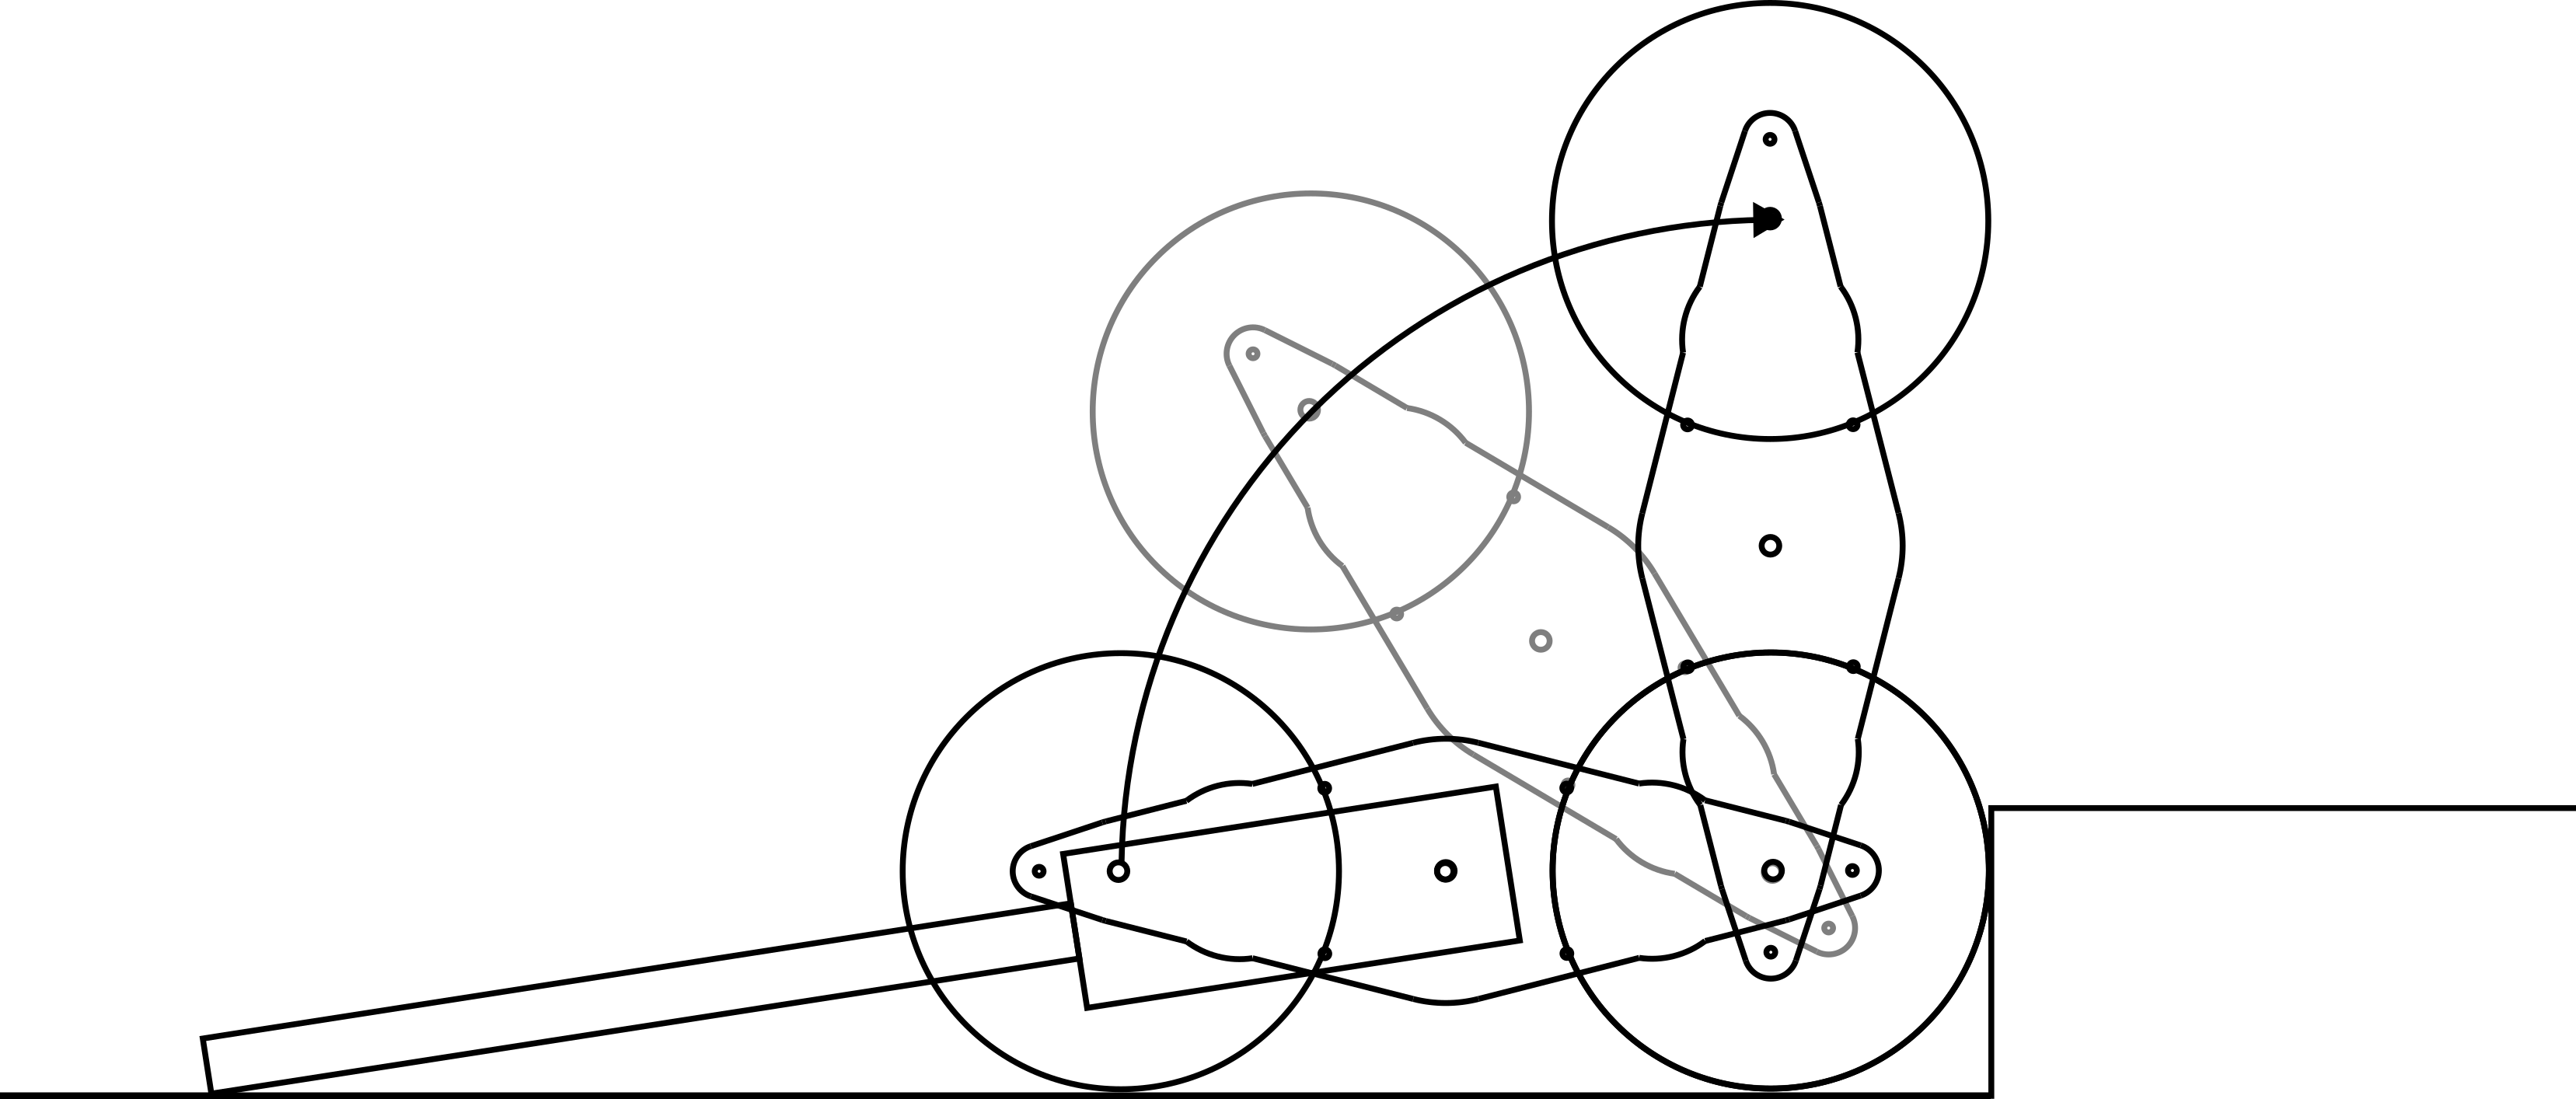
\includegraphics[width=0.35\textwidth]{FBDs/Stage-1}
	\caption{Stage 1 motion.}
	\label{fig:stage1}
\end{wrapfigure}
When the front wheels of the LIMs come into contact with the first step, they are blocked by a step and fixed in place. The tail pushes against the ground and the LIMs start rotating up the step. This motion ends when the LIMs are vertical.
\\
\subsection*{Stage 2: Flipping}
\begin{wrapfigure}{r}{0.35\textwidth} %this figure will be at the left
	\centering
	\includegraphics[width=0.35\textwidth]{FBDs/Stage-2}
	\caption{Stage 2 motion.}
	\label{fig:stage2}
\end{wrapfigure}
Once the LIMs are vertical, the bottom wheels start to roll backwards as the top wheels fall forward onto the step. The distance that the bottom wheels roll depends on the speed of the LIMs and the height of the step. If the frames of the LIMs hits the edge of the step, the device may slip backwards until the top wheel makes contact with the step. This motion ends when the top wheel is on the step.\\

\subsection*{Stage 3: Climbing}
\begin{wrapfigure}{r}{0.35\textwidth} %this figure will be at the left
	\centering
	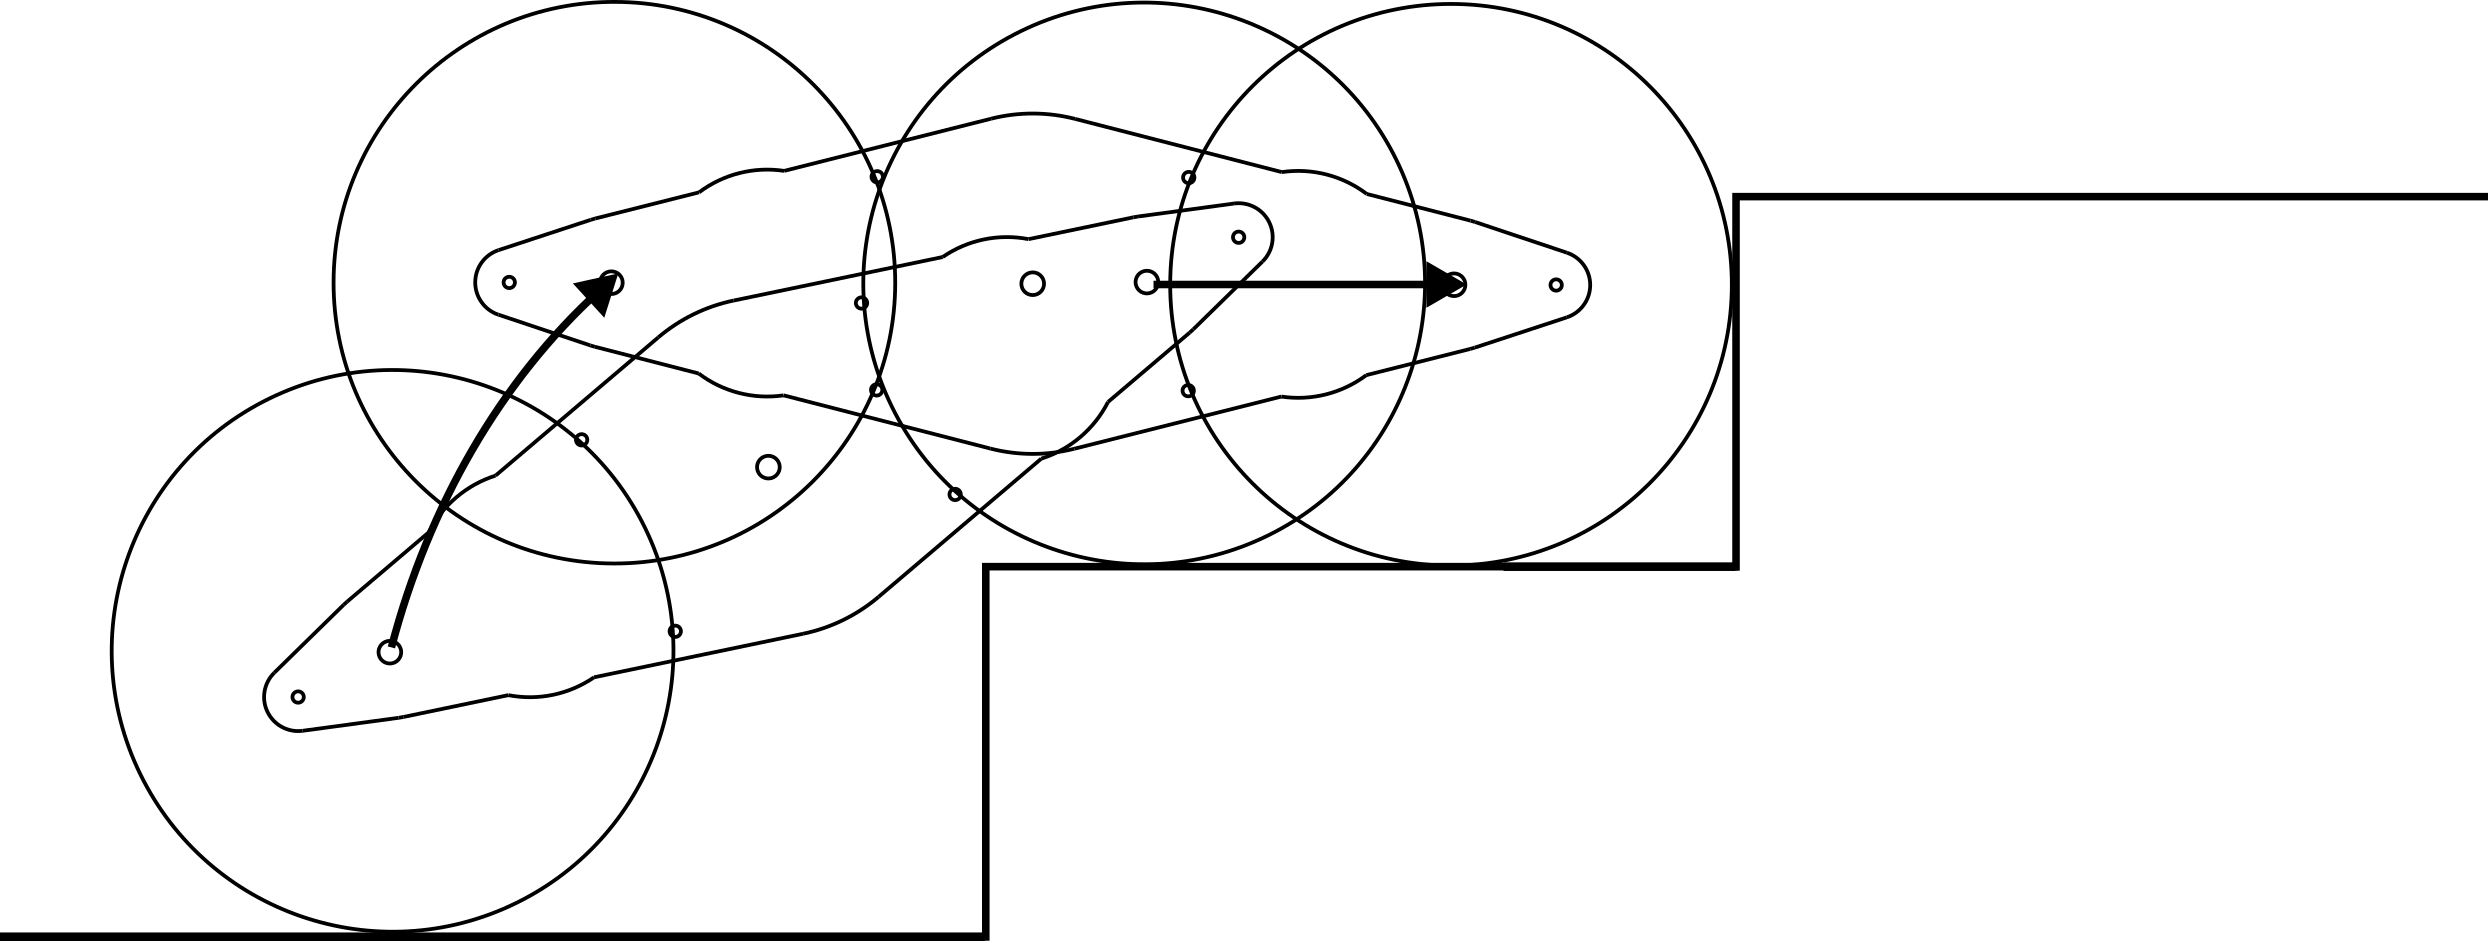
\includegraphics[width=0.35\textwidth]{FBDs/Stage-3}
	\caption{Stage 3 motion.}
	\label{fig:stage3}
\end{wrapfigure}
The front wheel rests on the step while the back wheel is on the ground. The tail pushes against the ground and the back wheel lifts while the front wheel simultaneously rolls forward on the step. This motion ends when the front wheel reaches the next step.\\

Stages 1 to 3 will repeat until the tail leaves the ground. After this point the tail will push against the edge of the previous steps. The number of steps the device must climb before the tail leaves the ground will depend on the length of the tail, the size of the other components, and the size of the steps. 

\subsection*{Stage 4: Lifting from step}
\begin{wrapfigure}{r}{0.35\textwidth} %this figure will be at the left
	\centering
	\includegraphics[width=0.35\textwidth]{FBDs/Stage-4}
	\caption{Stage 4 motion.}
	\label{fig:stage4}
\end{wrapfigure}
Similar to Stage 1, but the tail pushes against the edge of a previous step, which now applies a force pulling the device backwards. Assuming friction on the wheel is sufficient, the LIMs start rotating up the step. This motion ends when the LIMs are vertical.

\subsection*{Stage 5: Flipping from step}

Similar to Stage 2, but the tail pushes against the edge of a previous step, which now applies a force pulling the device backwards. This motion ends when the top wheel is on the step.\\
\begin{figure}[!h] %this figure will be at the left
	\centering
	\includegraphics[width=0.4\textwidth]{FBDs/Stage-5}
	\caption{Stage 5 motion.}
	\label{fig:stage5}
\end{figure}
\subsection*{Stage 6: Climbing from step}

\begin{wrapfigure}{r}{0.35\textwidth} %this figure will be at the left
	\centering
	\includegraphics[width=0.35\textwidth]{FBDs/Stage-6}
	\caption{Stage 6 motion.}
	\label{fig:stage6}
\end{wrapfigure}

Similar to Stage 3, but the tail pushes against the edge of a previous step, which now applies a force pulling the device backwards. The back wheel lifts while the front wheel rolls forward on the step. This motion ends when the front wheel reaches the next step.\\


\section{Core equations and assumptions}

The maths model is a system of equations that are solved simultaneously. These equations are derived from the free body diagrams of each component, and only consider movement in two dimensions. The components in question are the LIM frame, the sun gear, the idler gears, and the planet gears including the shaft and the wheels, and the body of the device. These components make contact with the surroundings and the other components, which exert equal and opposite forces on each other. As the maths model only considers movement in two dimensions, the LIMs are assumed to move synchronously. To simplify the equations, only one LIM is modelled, and its mass and moment of inertia is doubled.\\

Consider the device climbing a step as visualised in Figure \ref{Component-names}. Each component is assigned a number, where the LIM frame is 1, the sun gear is 2, the idler gears are 3 and 4, the planet gears, including the wheels, are 5 and 6, and the body of the device, including the tail, is 7.
\begin{figure}[h]
	\centering
	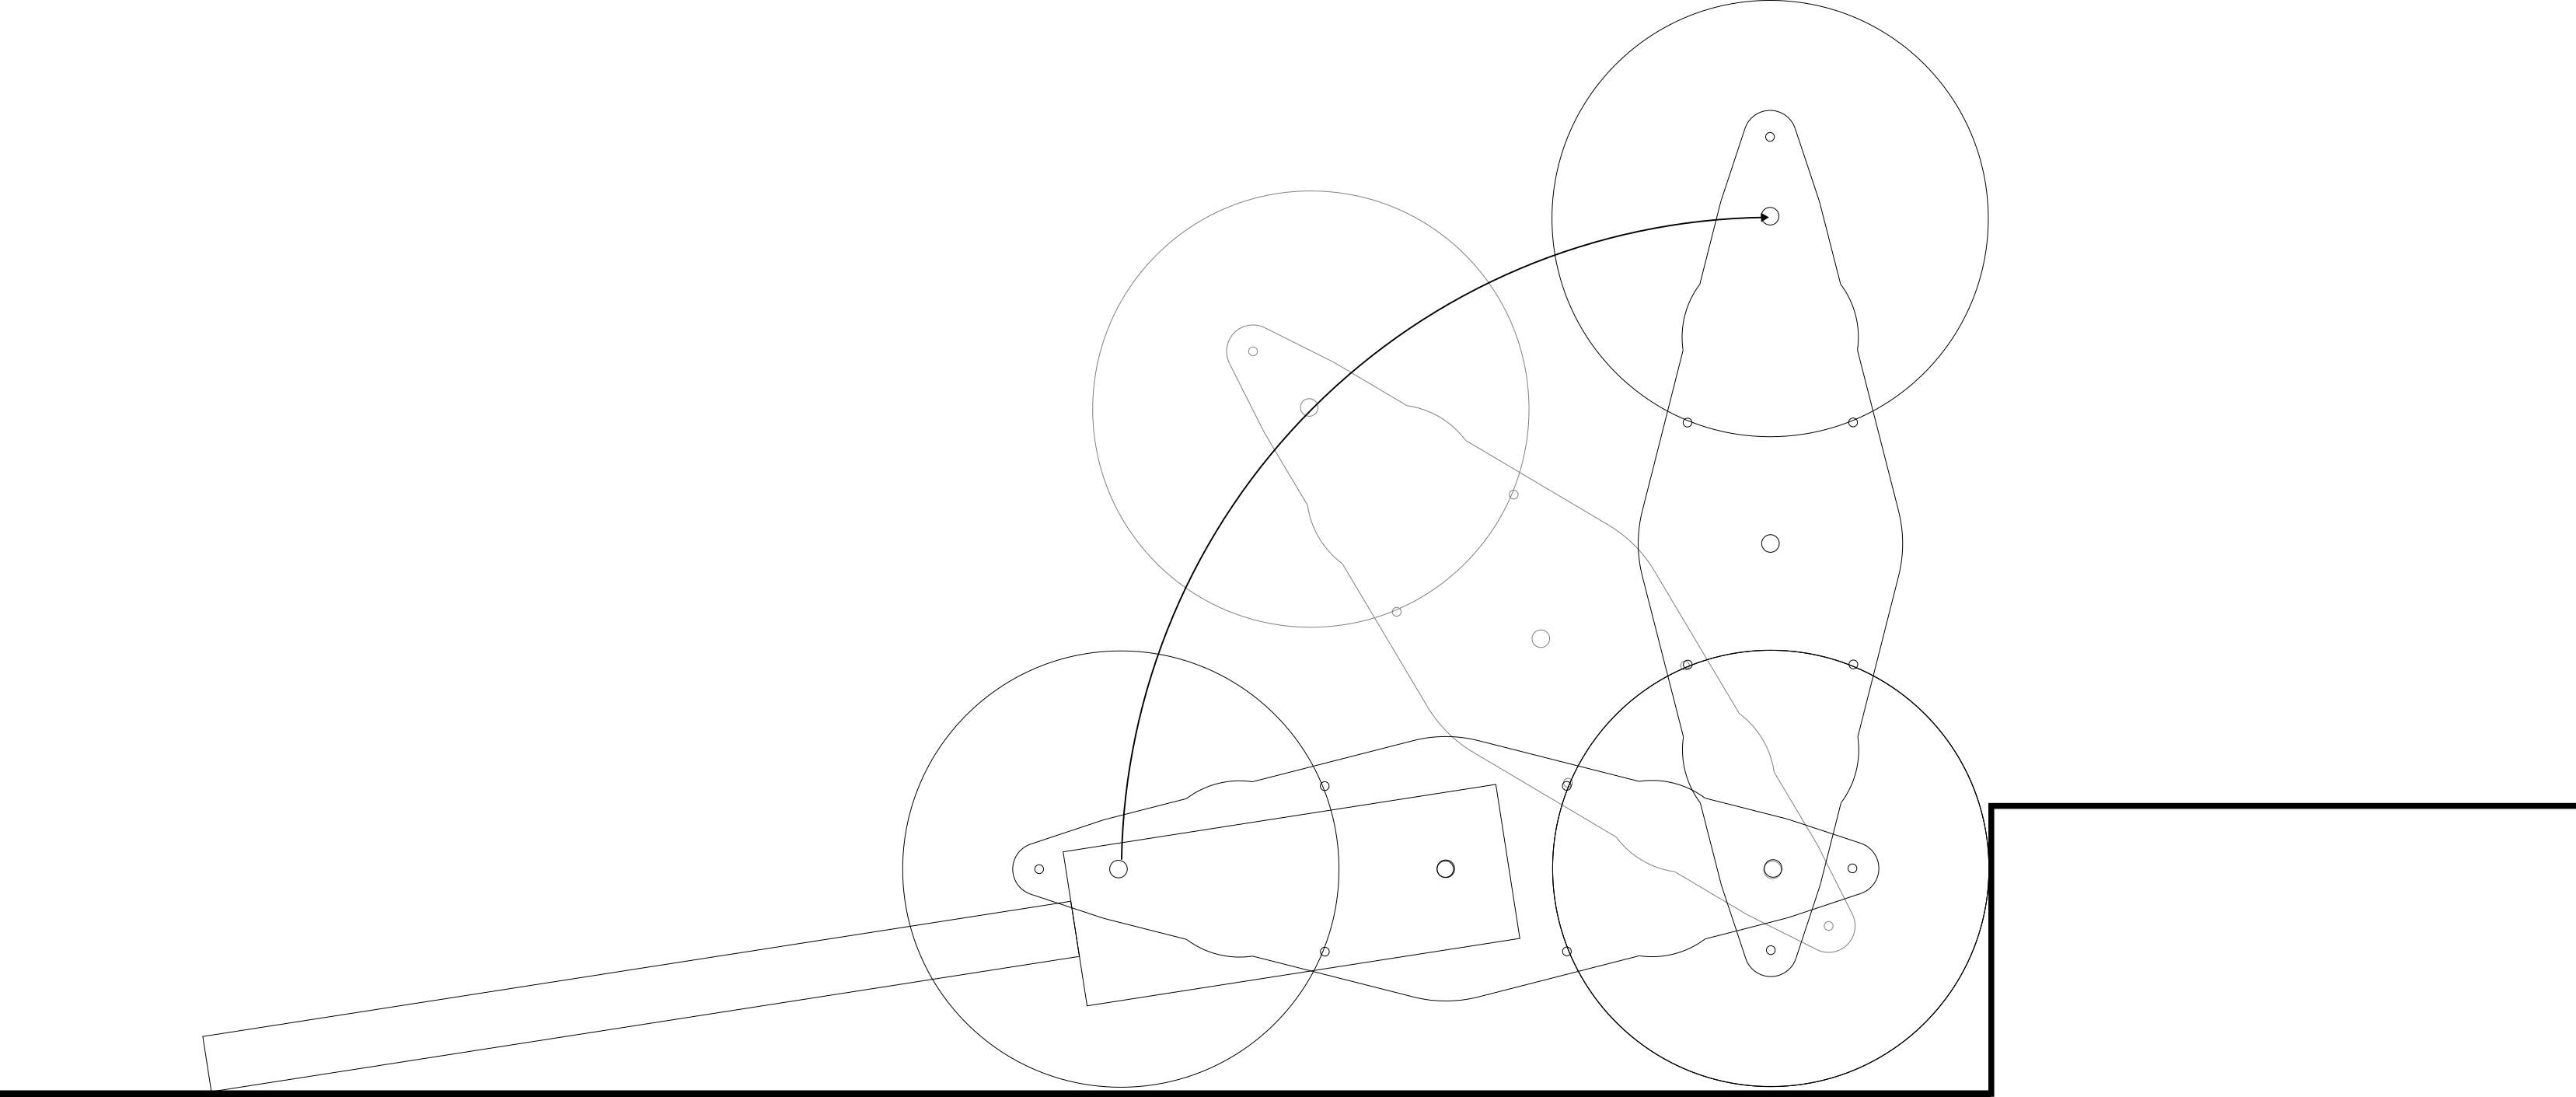
\includegraphics[width=0.7\textwidth]{FBDs/Naming components.png}
	\caption{Labelled components.}
	\label{Component-names}
\end{figure}
Powering the motor causes a torque between the body of the device and the sun gear. The components of the device that make contact with the environment, namely the front wheel and the tail, will be subject to external reaction forces, which are dependent on the stage of motion. These forces and torques will propagate internally through the gears, causing a forward motion. The free body diagrams for each component are shown in Figures \ref{FBD-1} and \ref{FBD-2}.\\
\begin{figure}[h]
	\centering
	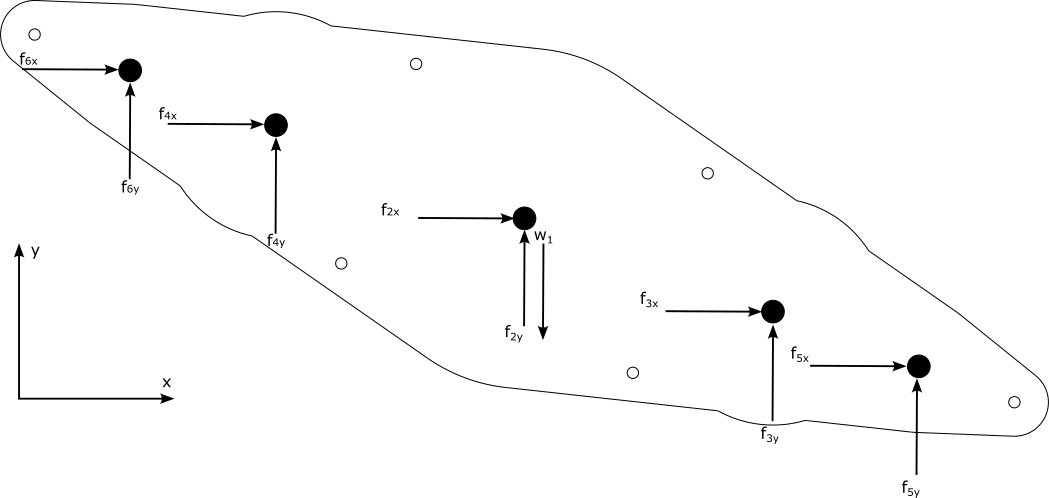
\includegraphics[width=0.8\textwidth]{FBDs/FBD-1.png}
	\caption{Free body diagram of the LIM frame (component 1).}
	\label{FBD-1}
\end{figure}
\begin{figure}[!h]
	\centering
	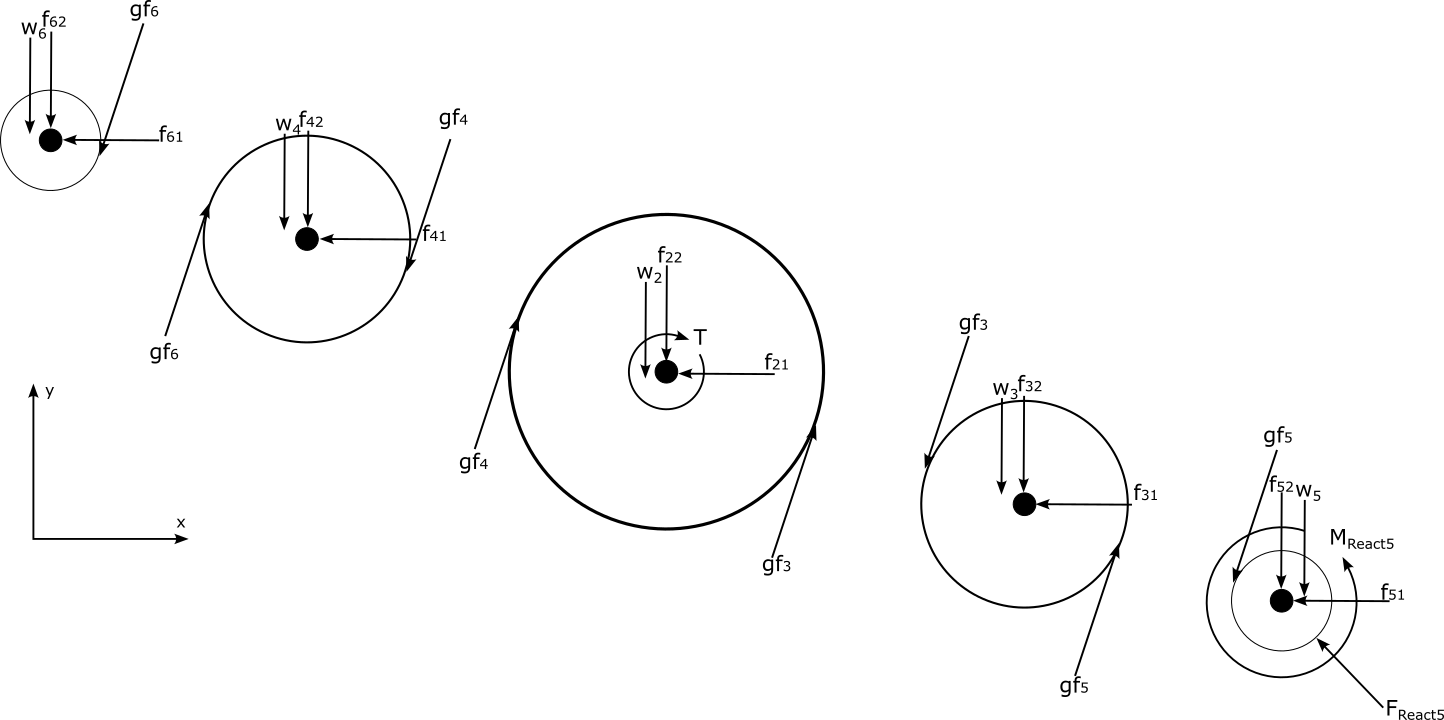
\includegraphics[width=0.8\textwidth]{FBDs/FBD-2.png}
	\caption{Free body diagram of the gears (components 2-5).}
	\label{FBD-2}
\end{figure}

Each component exerts a force on connected components, which exert an equal and opposite force back.
For example, the sum of forces equations for the sun gear are,\\
\begin{equation}
	m_2\vec{a_2} = \vec{w_2}-\vec{f_2}+\vec{\mathrm{gf}_3}+\vec{\mathrm{gf}_4}
\end{equation}
Where $m_n$ refers to the mass of component $n$, $\vec{a_n}$ is the acceleration vector of component $n$, $\vec{w_n}$ is the weight vector of component $n$, $\vec{f_n}$ is the force vector that component $n$ applies to component 1,  and $\vec{\mathrm{gf}_3}$ and $\vec{\mathrm{gf}_4}$ are the force vectors that components 3 and 4 respectively apply to component 2 through the gears.
This can be expanded to,
\begin{equation}
	m_2
	\begin{bmatrix}
		a_{2x}\\
		a_{2y}\\
		a_{2z}\\
	\end{bmatrix}
	=
	\begin{bmatrix}
		w_{2x}-f_{2x}+\mathrm{gf}_{3x}+\mathrm{gf}_{4x}\\
		w_{2y}-f_{2y}+\mathrm{gf}_{3y}+\mathrm{gf}_{4y}\\
		w_{2z}-f_{2z}+\mathrm{gf}_{3z}+\mathrm{gf}_{4z}\\
	\end{bmatrix}
\end{equation}
where vector positions 1, 2, and 3 denote the x, y, and z dimensions respectively. This equation can be further simplified by restraining movement to the x and y dimensions, and substituting $\vec{w_2} = \begin{bmatrix} 0 \\ m_2g & \\ \end{bmatrix}$,
\begin{equation}
	m_2
	\begin{bmatrix}
		a_{2x}\\
		a_{2y}\\
	\end{bmatrix}
	=
	\begin{bmatrix}
		-f_{2x}+\mathrm{gf}_{3x}+\mathrm{gf}_{4x}\\
		m_2g-f_{2y}+\mathrm{gf}_{3y}+\mathrm{gf}_{4y}\\
	\end{bmatrix}
\end{equation}
Similarly, the sum of moments equation for the sun gear is derived
\begin{equation}
	I_2\ddot{\theta_2} = T - r_2|\vec{\mathrm{gf}_3}| + r_2|\vec{\mathrm{gf}_3}|
\end{equation}
where $I_2$ is the moment of inertia of component 2, $\theta_2$ is the angle of component 2, $T$ is the moment exerted by the motor on component 2, and $r_2$ is the radius of component 2. Note that in this project, all angles and moments are given in the clockwise direction.
\\
The full list of equations can be found in MATLAB/Core\_equations.mat in the project repository \citep{repo}.



\section{Boundary conditions}
Depending on the stage of the climbing, components of the device will come into contact with different parts of the steps and at different angles. To model climbing in each stage, a set of equations defining the contact is given for each stage.\\
\subsection*{Stage 1: Lifting}
The front wheel, referred to as component 5, is locked in place by the reaction forces from the step, this leads to the condition,
\begin{subequations}
	\label{wheel1locked}
	\begin{align}
		\vec{a_5} &= \vec{0}\\
		\vec{v_5} &= \vec{0}\\
		\dot{\theta}_5 &= 0\\
		\ddot{\theta}_5 &= 0
	\end{align}
\end{subequations}
where $\vec{v_n}$ refers to the velocity of component $n$. \\
The front wheel must be placed into a two-dimensional coordinate system. In Stage 1, the front wheel can be on the ground or on one of the steps, so long as the tail can reach the ground, and the front wheel will always be pressed against the edge of the next step. Placing the origin at the start of the steps, the position of the front wheel can be defined as,
\begin{equation}
	\vec{s_5}
	=
	\begin{bmatrix}
		\mathrm{StepWidth}\cdot N-r_w\\
		\mathrm{StepHeight}\cdot N+r_w\\
		0
	\end{bmatrix}
\end{equation}
where $\vec{s_5}$ is the position vector of the centre of the front wheel, $N$ is the number of the step on which the wheel is placed, with $N = 0$ placing the step on the ground, and $r_w$ is the radius of the wheel.\\
The end of the tail pushes against the ground, which leads to the following conditions,
\begin{subequations}
	\label{tailonground}
	\begin{align}
		s_{7\mathrm{end}y} &= 0\\
		F_{\mathrm{React}7x} &=  -\mu_{\mathrm{tail}}F_{\mathrm{React}7y}\\
		-\ddot{\theta_7} &= \frac{(|\vec{l_7}|^2 - l_{7y}^2)a_{1y} + l_{7y}v_{1y}^2}{|\vec{l_7}|^3 (1 - \frac{l_{7y}^2}{|\vec{l_7}|^2})^{3/2}} \label{tailongroundkinematics}
	\end{align}
\end{subequations}
where $s_{7\mathrm{end}y}$ is the y position of the endpoint of the tail, $F_{\mathrm{React}7x}$ and $F_{\mathrm{React}7y}$ are the reaction forces exerted onto the tail by the ground in the x and y dimensions respectively, $\mu_{\mathrm{tail}}$ is the coefficient of friction between the tail and the ground, $\vec{l_7}$ is the position of the end of the tail relative to the motor axle, and $l_{7y}$ is the component of $\vec{l_7}$ in the y dimension. \\
Equation \ref{tailongroundkinematics} is derived from,

\begin{subequations}
	\begin{align}
		-\theta_7(t) &= \arcsin{\frac{l_{7y}(t)}{|\vec{l_7}|}}\\
		\frac{d^2}{dt^2}-\theta_7(t) &= \frac{d^2}{dt^2}\arcsin{\frac{l_{7y}(t)}{|\vec{l_7}|}}
	\end{align}
\end{subequations}
where $\theta_7$ and $l_{7y}$ are treated as functions of time, $t$. This relation can be seen in Figure \ref{fig:tailGround}. $v_{1y}$ and $a_{1y}$ refer to the velocity and acceleration of the motor axle in the y dimension, and are equivalent to $-\dot{l}_{7y}$ and $-\ddot{l}_{7y}$ respectively. These equations assume that the width of the tail is negligible.\\

\begin{figure}[!h]
	\centering
	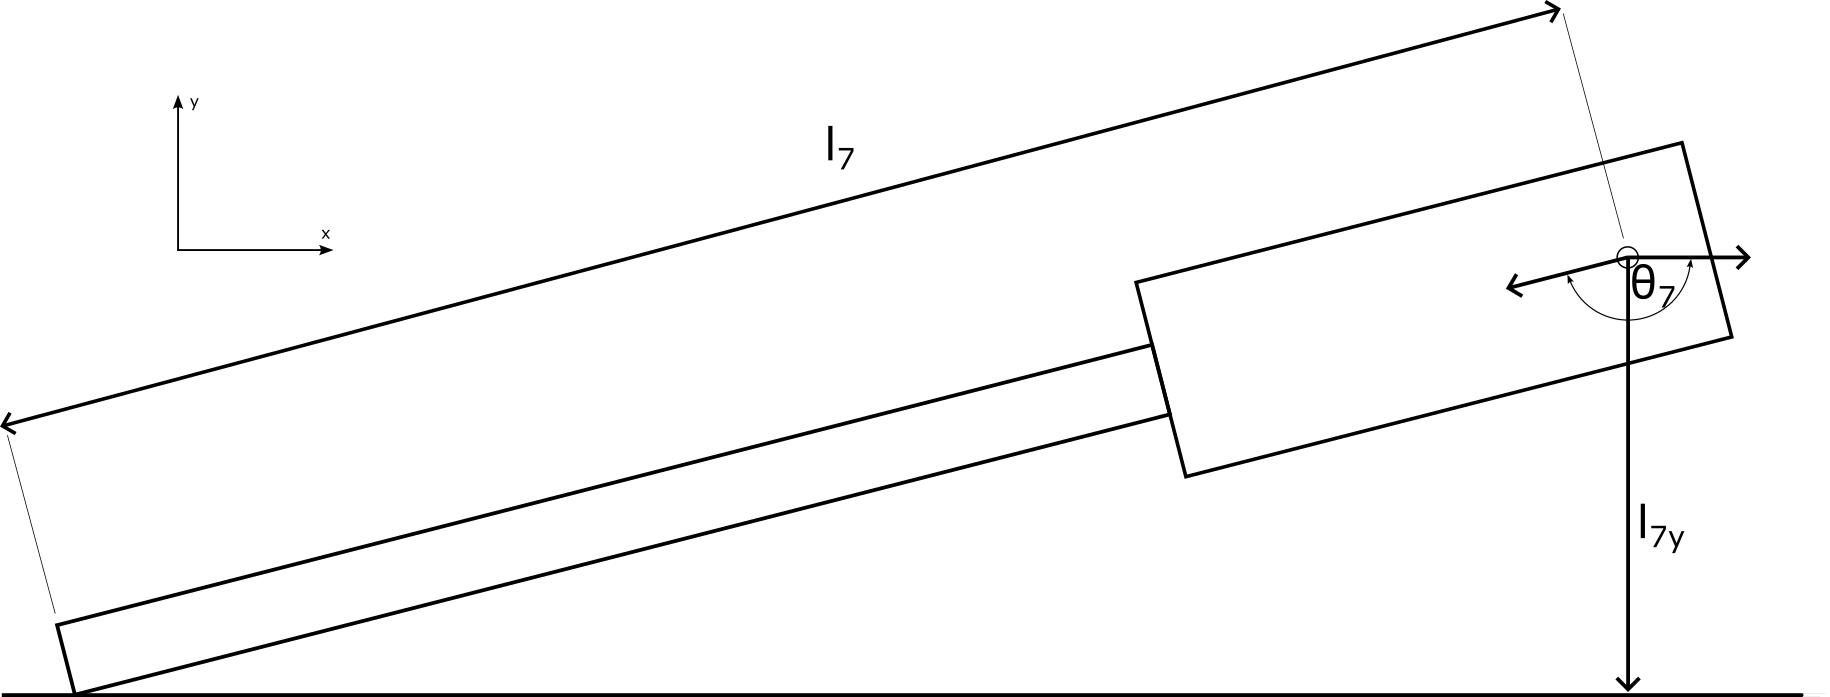
\includegraphics[width=0.8\textwidth]{FBDs/Tail-ground}
	\caption{Definition of $\vec{l}_7$ and $\theta_7$.}
	\label{fig:tailGround}
\end{figure}

\subsection*{Stage 2: Flipping}

Once the LIM is vertical, there is no longer a force pushing the bottom wheel forward into the step, instead it rolls backwards. This leads to a new condition,
\begin{subequations}
	\label{wheel1rolling}
	\begin{align}
		\vec{a_5} &= \begin{bmatrix}
			\ddot{\theta}_5 r_w \\
			0\\
			0
		\end{bmatrix}\\
		\vec{v_5} &= \begin{bmatrix}
			\dot{\theta}_5 r_w \\
			0\\
			0
		\end{bmatrix}\\
		s_{5x} &= \theta_{5} r_w;\\
		M_{\mathrm{React}5} &= - F_{\mathrm{React}5x} r_w;
	\end{align}
\end{subequations}
where $M_{\mathrm{React}5}$ is the reaction moment on wheel 5 as a result of the reaction forces.
The tail is still on the ground, so will still be subject to Equations \ref{tailonground}.

\subsection*{Stage 3: Climbing}

In Stage 3, the front and back wheel have swapped. To simplify the movements, component 5 will always refer to the wheel that makes contact with the steps, and component 6 will refer to the wheel that does not. \\
The front wheel is rolling and the tail is on the ground, which are the same conditions as in Stage 2. As such, Stage 3 is subject to Equations \ref{wheel1rolling} and \ref{tailonground}.

\subsection*{Stage 4: Lifting with tail on step}
Stage 4 is similar to Stage 1, except the tail is on the step. As such, this motion is subject to Equations \ref{wheel1locked} because the wheel is locked, and a set of new conditions because the tail is on the edge of the step,

\begin{subequations}
	\label{tailonstep}
	\begin{align}
		u_x &= \mathrm{StepWidth}\cdot (N_2-1)- s_{1x}\\
		u_y &= \mathrm{StepHeight}\cdot N_2 - s_{1y}\\
		\tan{(-\theta_7)} &= \frac{u_y}{u_x}\label{tailonstepposition}\\
		\begin{split}
		-\ddot{\theta_7} &= \frac{1}
		{(u_x^2 + u_y^2)^2}
		\Big( u_x^2 (a_{1x} u_y  - 2 v_{1x} v_{1y})
		+ u_y^2 (a_{1x} u_y + 2  v_{1x}  v_{1y}  )  \: ...\\
		&\;\;\;\;\;-  a_{1y} u_x^3 
		- u_x  u_y  (- 2  v_{1x}^2 + 2 v_{1y}^2 + a_{1y} u_x  )\Big)
		\end{split}
		\label{tailonstepaccelleration}\\
		F_{\mathrm{React}7x}' &= -\mu_{\mathrm{tail}} F_{\mathrm{React}7y}'\\
		\vec{F}_{\mathrm{React}7} &= \begin{bmatrix}
			-\cos{(\theta_7)} & -\sin{(\theta_7)} & 0\\
			\sin{(\theta_7)} & -\cos{(\theta_7)} & 0\\
			0 & 0 & 1
		\end{bmatrix} \vec{F}_{\mathrm{React}7}'
	\end{align}
\end{subequations}
where $N_2$ is the number of the step that the tail makes contact with, $\mathrm{StepWidth}$ and $\mathrm{StepHeight}$ are the width and height of each step in the stairs, $u_x$ and $u_y$ are the displacement from the motor axis to the point of contact between the tail and the step. Equation \ref{tailonstepaccelleration} is the second derivative of \ref{tailonstepposition}. $\vec{F}_{\mathrm{React}7}'$ is the vector of reaction forces in a rotated coordinate system such that $F_{\mathrm{React}7y}'$ is the normal force between the tail and the step.

\subsection*{Stage 5: Flipping from step}
Stage 5 is similar to Stage 2, except the tail is on the step. As such, this motion is subject to Equations \ref{wheel1rolling} because the wheel is locked, and Equations \ref{tailonstep} because the tail is on the step.\\

\subsection*{Stage 6: Climbing from step}
Stage 6 is similar to Stage 3, except the tail is on the step. As such, this motion is subject to Equations \ref{wheel1rolling} because the wheel is locked, and Equations \ref{tailonstep} because the tail is on the step.\\

\section{Solving technique}
The MATLAB symbolic toolbox comes with the solve() function, which can be used to solve sets of non-linear simultaneous equations. However, it struggles with this large set of equations that contain trigonometric functions, often stalling. This project develops a function that breaks down the set of equations into smaller, easier to solve sets, then substitutes these solutions into the remaining equations. Figure \ref{fig:solver-flowchart} shows the flowchart for this function. \\

\begin{figure}[!!h]
	\centering
	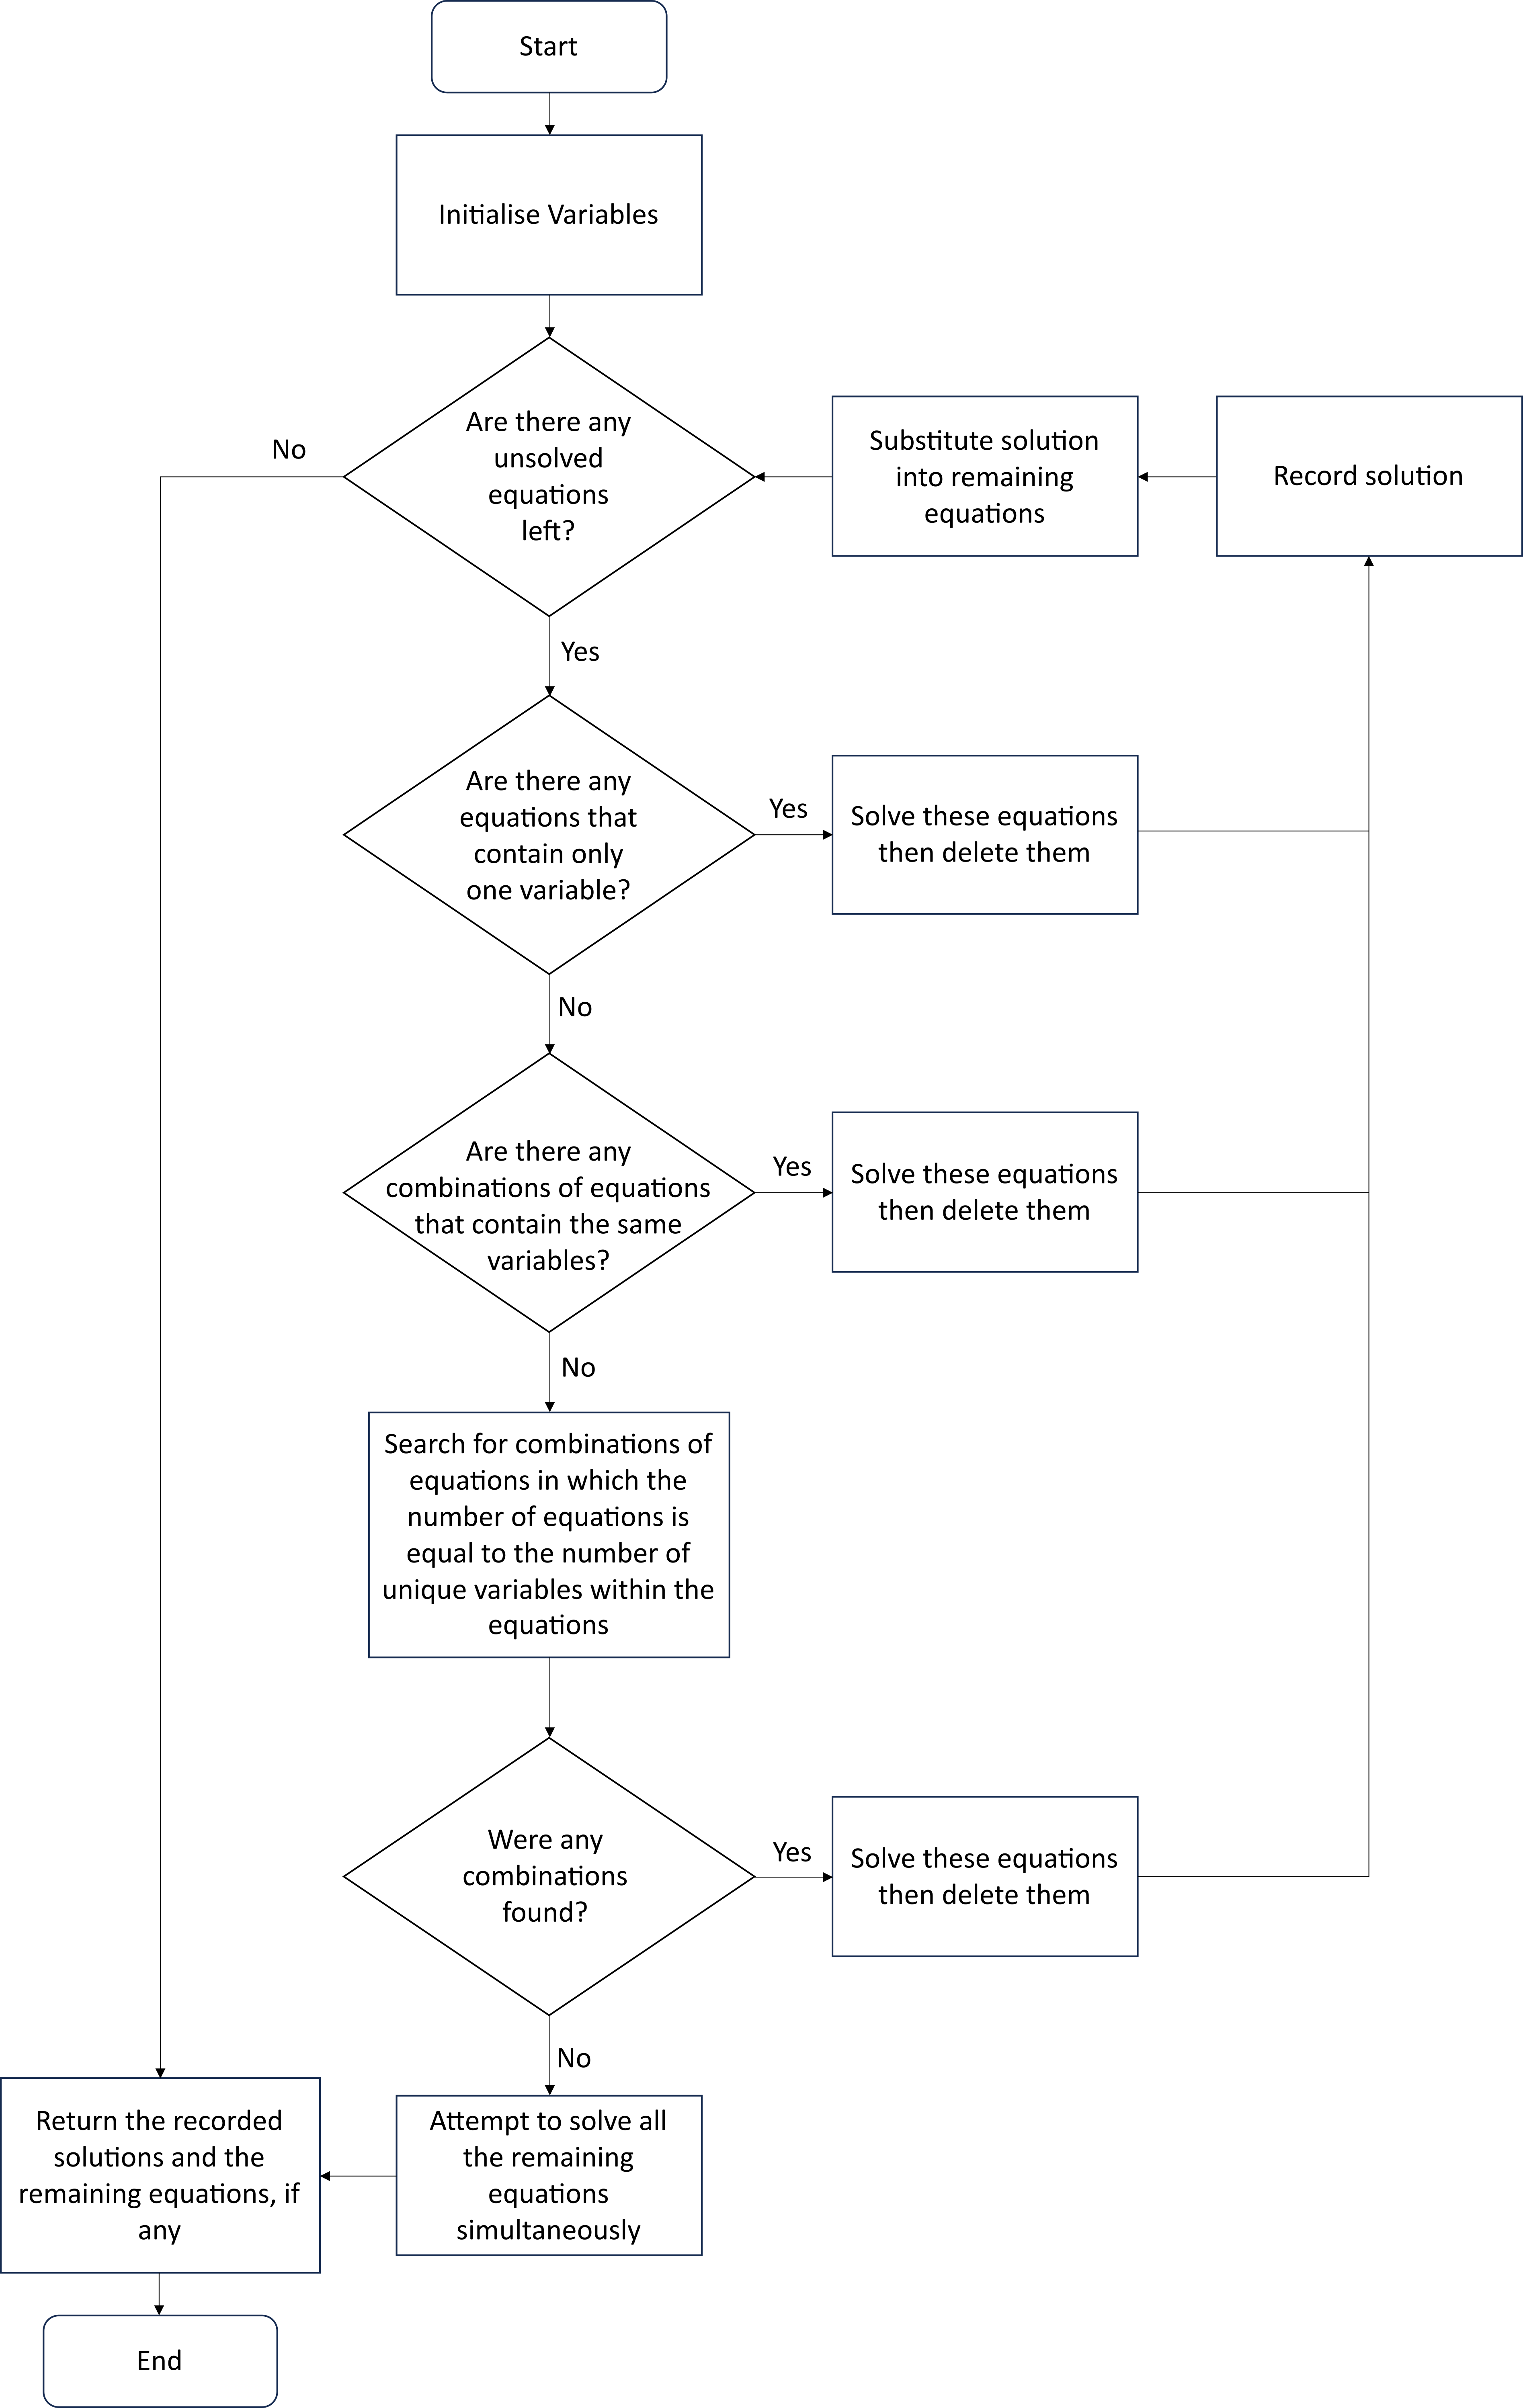
\includegraphics[height=0.9\textheight]{solver-flowchart}
	\caption{Flowchart for this project's solver.}
	\label{fig:solver-flowchart}
\end{figure}
The function loops through the equations until they have all been solved, or it cannot find any more solutions. First, it identifies any trivial equations that contain only one variable, such as $a = 1$, and solves them. This will also pick up equations with more than one solution, such as $\sin(a) = 1$; to resolve this, the solver will look for inequalities that contain the relevant variable, in this case $a$, and apply them to the solution. For example, if you were to provide the function with the set of equations:\\

\begin{subequations}
	\label{exampleinput}
	\begin{align}
		a &= 0.5 \label{example1a}\\
		\sin{(b)} &= a\\
		b &>= \frac{\pi}{2}\\
		b &<= \pi
	\end{align}
\end{subequations}
The first loop would identify Equation \ref{example1a} as it only has one variable. It wouldn't find any inequalities that describe the variable $a$ so it would simply send the equation $a = 0.5$ to MATLAB's solve() function. It then records the solution and substitutes it into the remaining equations, 
\begin{subequations}
	\label{example2}
	\begin{align}
		\sin{(b)} &= 0.5 \label{example2a}\\
		b &>= \frac{\pi}{2}\label{example2b}\\
		b &<= \pi\label{example2c}
	\end{align}
\end{subequations}
The second loop identifies Equation \ref{example2a} as it only has one variable. It looks for inequalities that describe $b$ and finds Inequalities \ref{example2b} and \ref{example2c}. It then sends all three to MATLAB's solve() function, which returns the solution for $b$.
The function then outputs a structure with the fields,
\begin{subequations}
	\begin{align}
		\mathrm{solution.a} &= 0.5\\
		\mathrm{solution.b} &= \frac{5\pi}{6}
	\end{align}
\end{subequations}

Once the function can no longer find trivial solutions, it looks for sets of equations that contain the exact same variables, such as equations of the form,
\begin{subequations}
	\begin{align}
		a -2b &= 0\\
		b -a +2 &= 0 
	\end{align}
\end{subequations}
and sends them to be solved. For this to work, there must be at least as many equations as there are variables in the set. This function will also identify and delete duplicate equations.\\
Once the function can no longer find sets of equations that use the exact same variables, it will attempt to find sets of equations that fully describe a set of variables, such as,
\begin{subequations}
	\begin{align}
		a -3b &= 0\\
		b -c +2&= 0\\
		a -2c &= 0
	\end{align}
\end{subequations}
Finally, if it can't find any fully defined sets up to a certain size, it will attempt to solve the complete set of remaining equation using the solve() function. If the function is unable to solve all the equations, it will return a structure containing the solutions it has found, and a vector containing the remaining equations. This is useful for debugging as it provides feedback on which variables it did and did not have enough information to solve for, something the MATLAB solve() function does not do.\\


\section{Required torque}
When designing a LIM robot, it is essential to size the motor and gearbox to be able to provide enough torque to lift the LIMs. To do this, one must first determine which stage of motion requires the most torque. To find the minimum torque required to cause forward movement, we solve for the torque that results in an overall acceleration of 0 when the velocity is also 0, essentially adding the conditions:
\begin{subequations}
	\label{condition-static}
	\begin{align}
		\vec{a} &= \vec{0}\\
		\vec{v} &= \vec{0}\\
		\ddot{\theta_1} &= 0\\
		\dot{\theta_1} &= 0\\
	\end{align}
\end{subequations}
which simplifies the dynamic equations into static equations.\\
The set of equations is then solved for a range of positions in each stage. The required torque across the full range of motion is shown in Figure \ref{fig:bigplot}, along with illustrations of the device as it transitions between stages of motion. Figure \ref{fig:bigplot} shows that the highest torque is needed for the Stage 4 motion.\\


\begin{figure}[h]
	\centering
	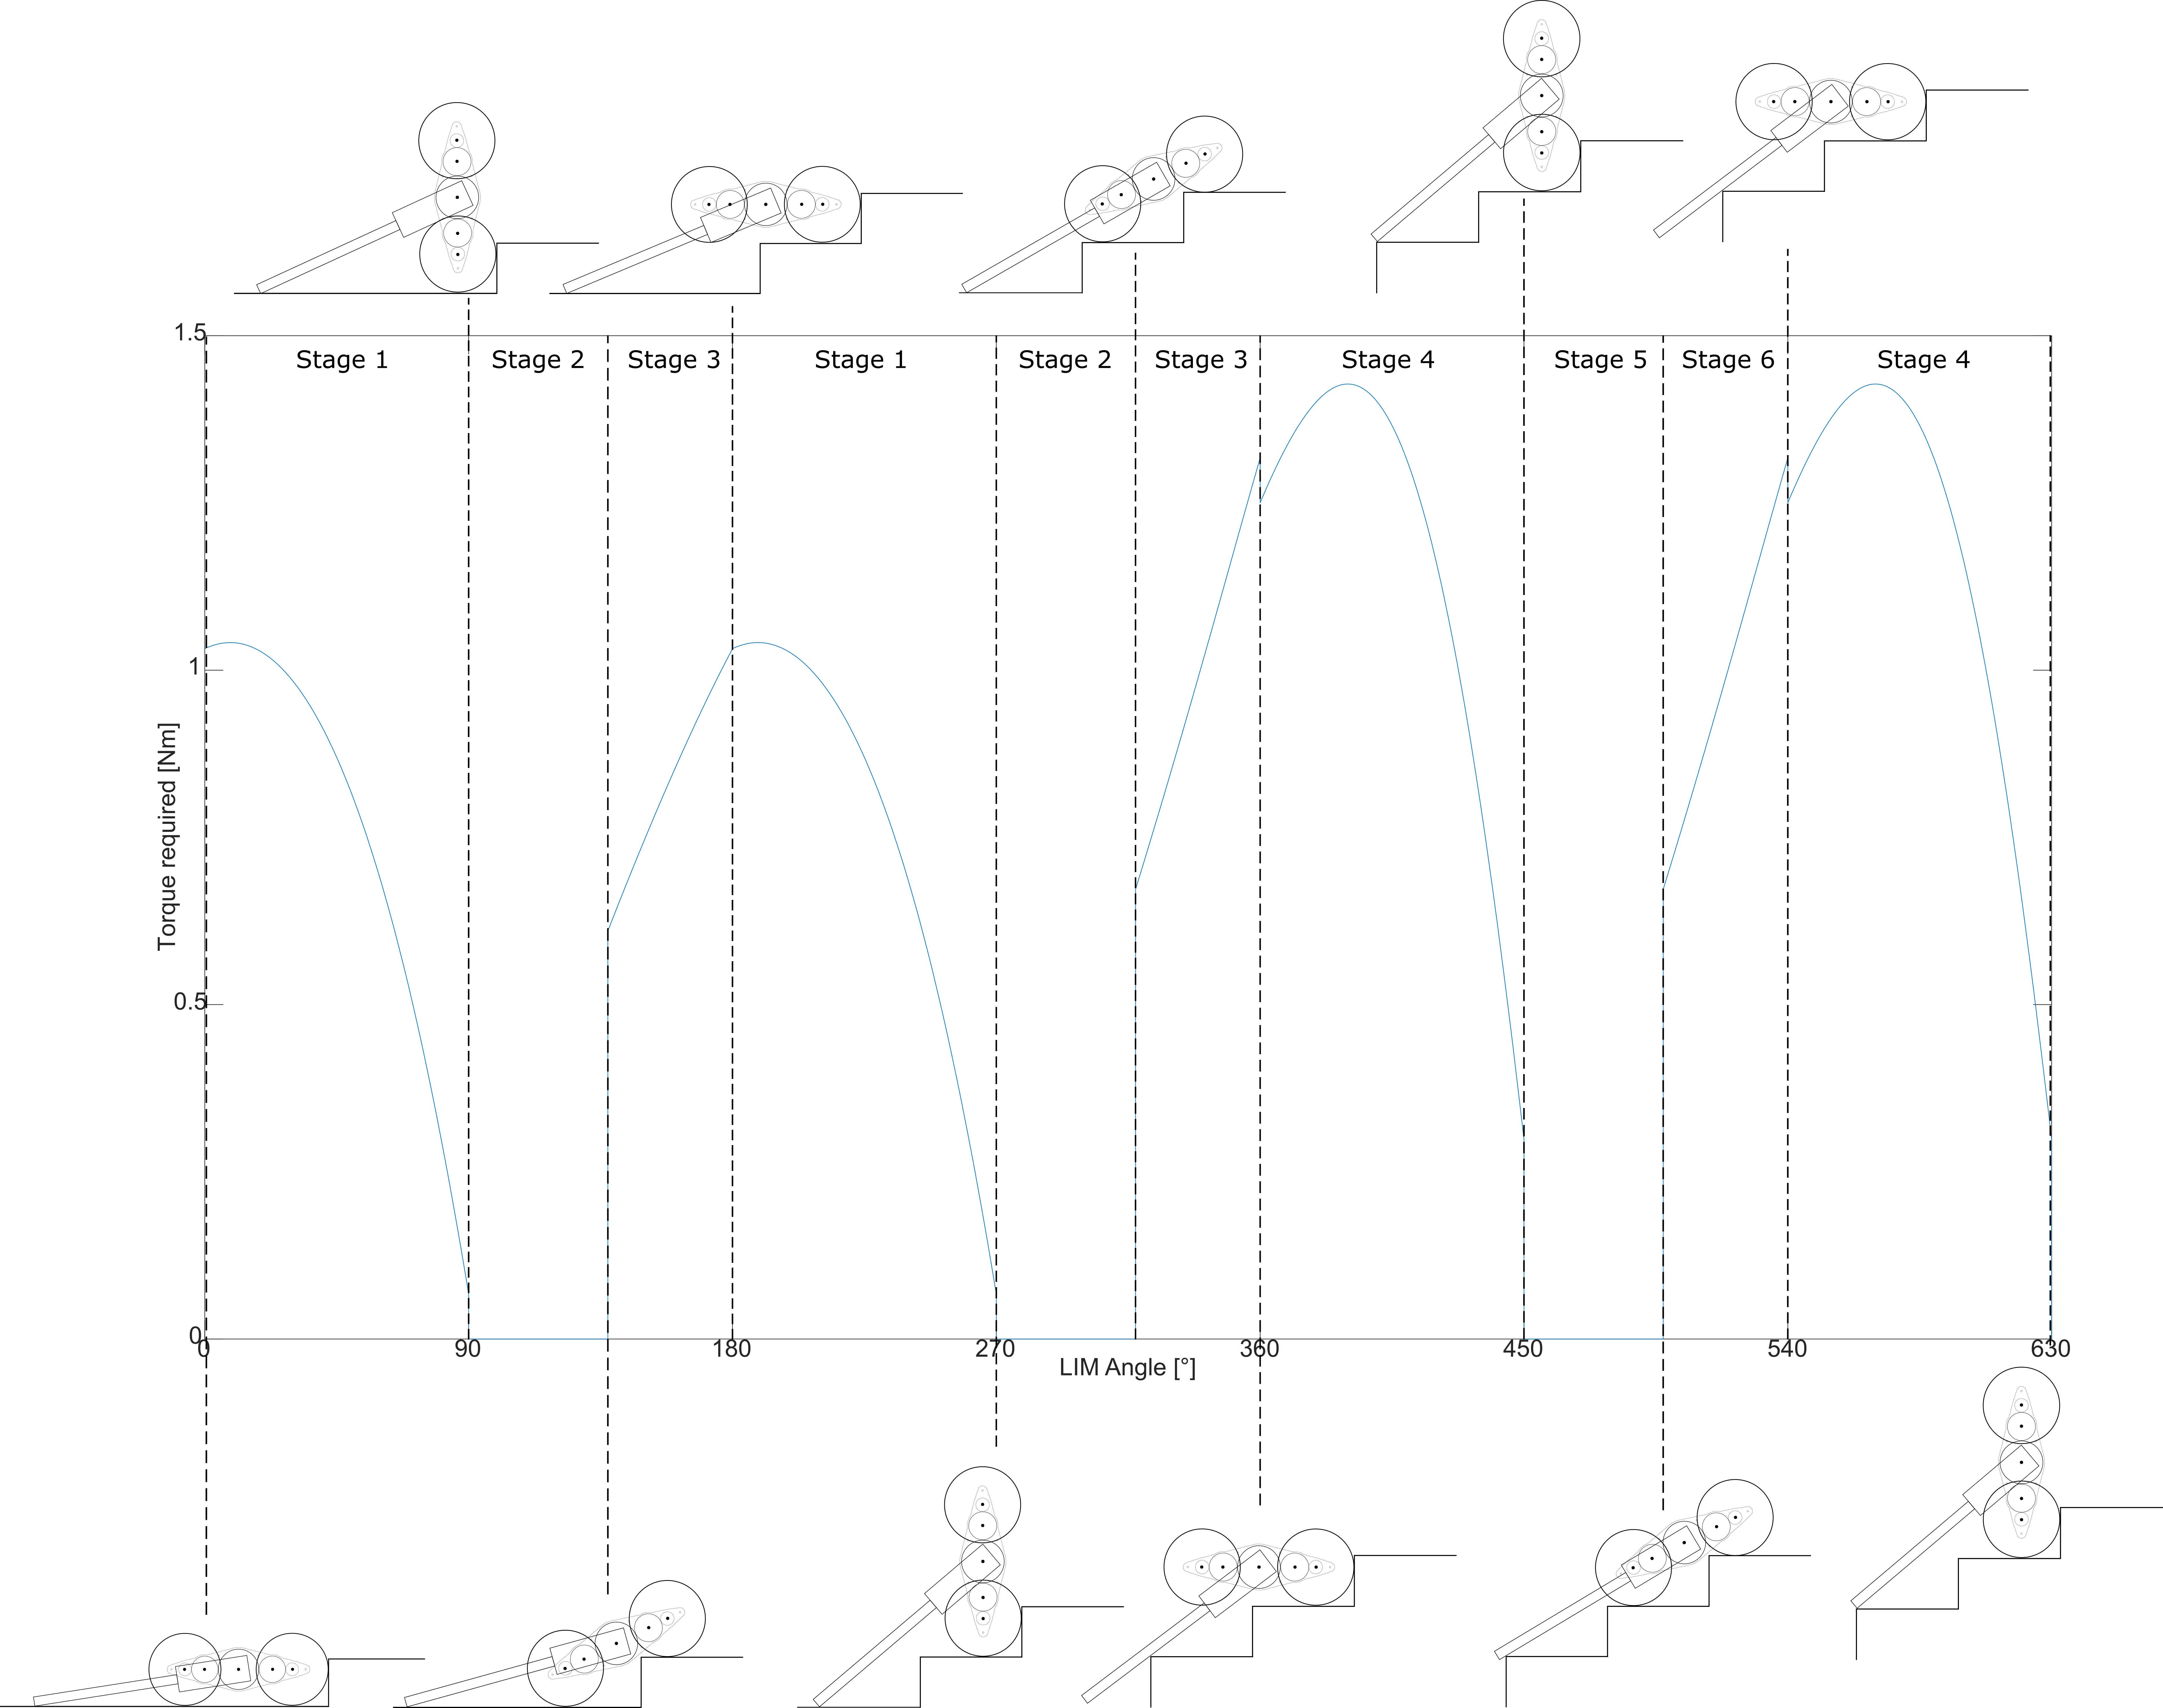
\includegraphics[width=1\textwidth]{plots/bigplot}
	\caption{Relationship between LIM angle and required torque across all stages of motion.}
	\label{fig:bigplot}
\end{figure}

During Stages 1 and 4, the required torque increases slightly as the LIM lifts up from horizontal, then rapidly decreases as the LIM approaches vertical. During Stages 2 and 5, the LIM simply falls down onto the next step, so no motor torque is required. During Stages 3 and 6, the required motor torque gradually increases as the back wheel of the LIM lifts and the front wheel rolls to the next step. 

\section{Required coefficient of friction}

When the device climbs steps, it is possible that the front wheel, component 5, will slip. Slipping can cause the device to be unable to climb stairs, and the maths model works under the assumption that there is no slipping. Applying the Coulomb approximation of friction to the model, slipping will occur when $|F_{5x}| > \mu_5 F_{5y}$, where $\mu_5$ is the coefficient of friction between the wheel and the step. This coefficient can be increased by using certain materials, such as rubber, for the contact surface of the wheels. However, the coefficient of friction is also dependent on the material of the step itself, which a designer would not have control over. For this reason, designers may want to modify the design to reduce the required coefficient of friction.\\
Similar to the required torque, the coefficient of friction required to prevent slipping can also be calculated across the motion, and the highest value is in Stage 4, as seen in Figure \ref{bigplot-grip}.

\begin{figure}[h]
	\centering
	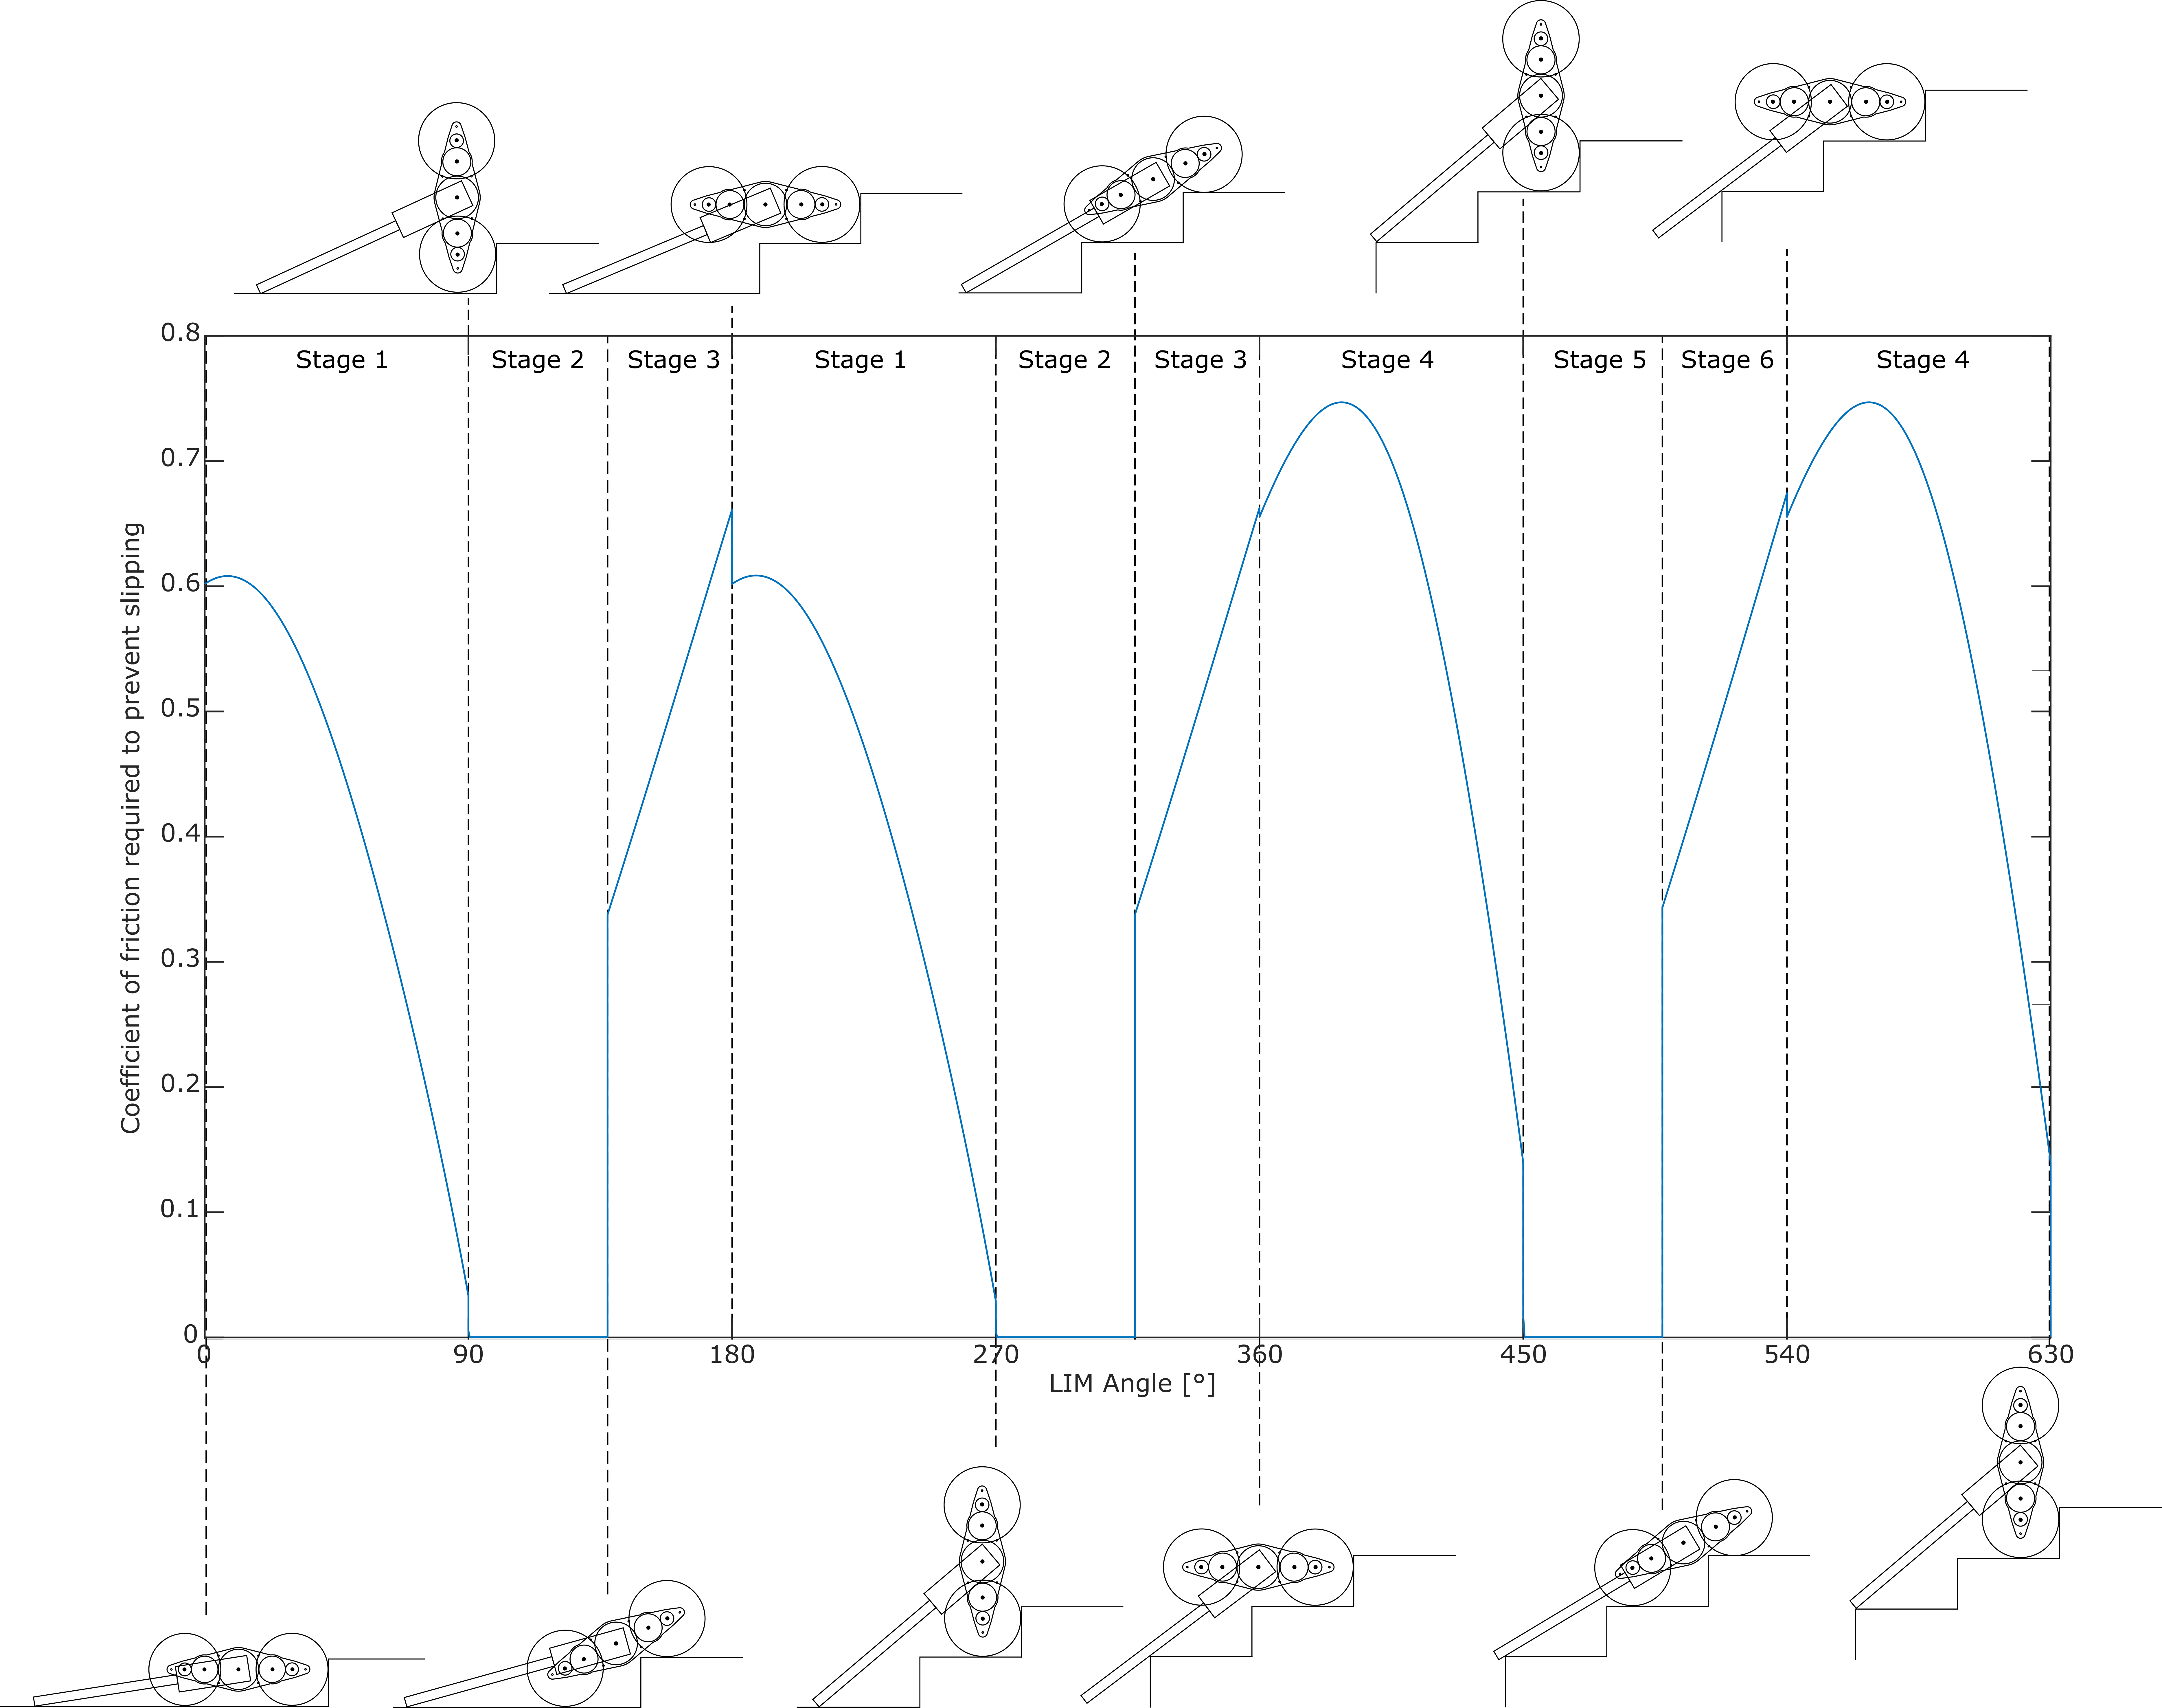
\includegraphics[width=1\textwidth]{plots/bigplot-grip}
	\caption{Relationship between LIM angle and required coefficient of friction.}
	\label{bigplot-grip}
\end{figure}

\section{Using the model to size components}
So far this section has only modelled a device with fixed parameters, such as gear ratio, wheel size, mass, and tail length, however a designer may be interested in varying these parameters. The model can be used to inform the design process by showing the effect that changing certain parameters has on the required torque and the required coefficient of friction. Both of these requirements are highest in Stage 4. For example, Figures \ref{fig:GR-torque} and \ref{fig:GR-friction} show how changing the gear ratio affects the required torque and required coefficient of friction respectively.\\

\begin{figure}[h]
	\centering
	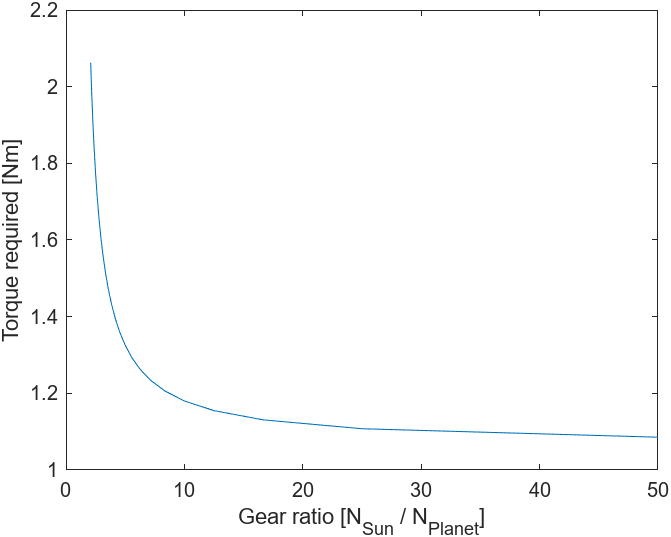
\includegraphics[width=0.8\textwidth]{plots/GR-torque}
	\caption{Relationship between LIM gear ratio and required torque.}
	\label{fig:GR-torque}
\end{figure}
\begin{figure}[h]
	\centering
	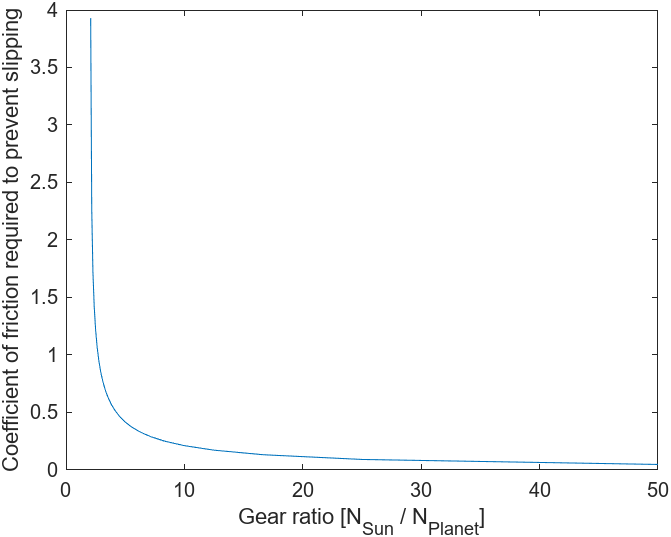
\includegraphics[width=0.8\textwidth]{plots/GR-friction}
	\caption{Relationship between LIM gear ratio and required coefficient of friction.}
	\label{fig:GR-friction}
\end{figure}
These plots show that maximising the ratio between the sun and planet gears will reduce the amount of torque required from the motor to allow forward movement, and allow the the device to climb without slipping on a larger range of surfaces. Interestingly, increasing the gear ratio will also allow the device to move faster when rolling without obstructions. This provides a useful insight for design, the device will be faster, need a less powerful motor, and slip less often with a higher gear ratio.
